\documentclass{article}

\usepackage{amsmath, amsthm}
\usepackage{setspace}
\usepackage{microtype, parskip}
\usepackage[comma,sort&compress]{natbib}
\usepackage{lineno}
\usepackage{docmute}
\usepackage{caption, subcaption, multirow, morefloats, rotating}
\usepackage{wrapfig}

\frenchspacing

\doublespacing

\raggedright

\begin{document}
\linenumbers
\modulolinenumbers[2]

%\maketitle

\begin{titlepage}
  \begin{large}
    \textbf{Title:} The interplay between extinction intensity and selectivity: correlation in trait effects on taxonomic survival
  \end{large}

  \textbf{Running title:} Variation in trait effects on taxonomic survival

  \textbf{Author:} Peter D Smits, psmits@uchicago.edu, Committee on Evolutionary Biology, University of Chicago, IL, USA.

  \textbf{Keywords:} macroevolution, extinction, macroecology, Bayesian, brachiopods

  \textbf{Word count:} 
  
  \textbf{Table count:} 2
 
  \textbf{Figure count:} 6

  \textbf{Data archival location:} If accepted, all data and code necessary to duplicate this analysis will be made available on DRYAD.

\end{titlepage}

\begin{abstract}
  While the effect of geographic range on extinction risk is well documented, how other traits may increase or decrease extinction risk is less well known. I analyze patterns of Paleozoic brachiopod genus durations and their relationship to geographic range, affinity for epicontinental seas versus open ocean environments, and body size. Additionally, I allow for environmental affinity to have a nonlinear effect on duration. Using a hierarchical Bayesian approach, I also model the interaction between the effects of biological traits and a taxon's time of origination. My analysis framework eschews the traditional distinction between background and mass extinction, and instead the entire time period is analyzed as parts of the same continuum. 
  
  These results support the hypothesis that as extinction intensity increases, overall extinction selectivity decreases.
\end{abstract}


\section{Introduction}

How do biological traits affect extinction risk? Biological traits are defined here as descriptors of a taxon's adaptive zone, which is the set of all biotic--biotic and biotic--abiotic interactions that a taxon can experience \citep{Simpson1944}. In effect, these are descriptors of a taxon's broad-sense ecology. \citet{Jablonski1986} observed that during a mass extinction event, the effects of biological traits on taxonomic survival decreased in size. However, this pattern was not the case for the effect of geographic range on survival \citep{Jablonski1986}. 

\citet{Jablonski1986} phrased his conclusions in terms of background versus mass extinction, but this scenario is readily transferable to a continuous variation framework as there is no obvious distinction in terms of extinction rate between these two states \citep{Wang2003}. Additionally, the \citet{Jablonski1986} scenario has strong model structure requirements in order to test its proposed macroevolutionary mechanism; not only do the taxon trait effects need to be modeled, but the correlation between trait effects need to be modeled as well. 

There are two end-member macroevolutionary mechanisms which may underlie the pattern observed by \citet{Jablonski1986}: the effect of geographic range on predictive survival remains constant and those of other biological traits decrease, or the effect of geographic range in predicting survival increases and those of other biological traits stay constant. Reality, of course, may fall somewhere along this continuum. % add more here

Conceptually, taxon survival can be considered an aspect of ``taxon fitness'' along with expected lineage specific branching/origination rate \citep{Cooper1984,Palmer2012}. A taxon with a beneficial trait should persist for longer, on average, than a taxon without that beneficial trait. Here I model brachiopod taxon durations because trait based differences in extinction risk should manifest as differences in taxon durations. Brachiopods are an ideal group for this study as they are are well known for having an exceptionally complete fossil record \citep{Foote2000a}. I focus on the brachiopod record from most of the Paleozoic, from the start of the Ordovician (approximately 485 My) through the end Permian (approximately 252 My) as this represents the time of greatest global brachiopod diversity \citep{Alroy2010}.

The analysis of taxon durations, or time from origination to extinction, falls under the purview of survival analysis, a field of applied statistics commonly used in health care \citep{Klein2003} but has a long history in paleontology \citep{Simpson1944,Simpson1953,VanValen1973,VanValen1979,Smits2015,Crampton2016}. I adopt a hierarchical Bayesian survival modeling approach, which represents both a conceptual and statistical unification of the paleontological dynamic and cohort survival analytic approaches \citep{VanValen1973,VanValen1979,Raup1978,Raup1975,Foote1988,Baumiller1993,Simpson2006,Smits2015,Crampton2016,Ezard2012b}. By using a Bayesian framework I am able to quantify the uncertainty inherent in the estimates of the effects of biological traits on survival. 

\subsection{Factors affecting brachiopod survival}

Geographic range is widely considered the most important taxon trait for estimating differences in extinction risk at nearly all times, with large geographic range associated with low extinction risk \citep{Jablonski1986,Jablonski1987,Jablonski2003,Payne2007}, though \citet{Foote2013} find that this generalization does not hold in the Mesozoic. For the Paleozoic, however, I expect this to hold true for the entire period analyzed.

Epicontinental seas are a shallow-marine environment where the ocean has spread over the surface of a continental shelf with a depth typically less than 100m. In contrast, open-ocean coastline environments have much greater variance in depth, do not cover the continental shelf, and can persist during periods of low sea level. Because of this, it is strongly expected that taxa which favor epicontinental seas would be at great risk during periods of low sea levels, such as during glacial periods, when epicontinental seas are drained. During the Paleozoic (approximately 541--252 My), epicontinental seas were widely spread globally but declined over the Mesozoic (approximately 252--66 My) and have nearly disappeared during the Cenozoic (approximately 66--0 My) as open-ocean coastlines became the dominant shallow-marine setting \citep{Peters2008,Miller2009a,Johnson1974}. 

\citet{Miller2009a} demonstrated that during several mass extinctions taxa associated with open-ocean environments tend to have a greater extinction risk than those taxa associated with epicontinental seas. During periods of background extinction, however, they found no consistent difference between taxa favoring either environment. These two environment types represent the primary environmental dichotomy observed in ancient marine systems \citep{Miller2009a,Peters2008,Sheehan2001b}. Given these findings, I predict that as extinction risk increases, the extinction risk associated with favoring open-ocean environments should generally increase. 

Because environmental preference is defined as the continuum between occurring exclusively in open-ocean environments versus epicontinental environments, intermediate values are considered ``generalists'' in the sense that they favor neither end member. A long standing hypothesis is that generalists or unspecialized taxa will have greater survival than specialists \citep{Simpson1944,Liow2004a,Liow2007b,Nurnberg2013a,Nurnberg2015,Baumiller1993}. Because of this, the effect of environmental preference was modeled as a quadratic function where a concave down relationship between preference and expected duration indicates that generalists are favored over specialists end-members.

Body size, measured as shell length, is also considered as a potential trait that influences extinction risk \citep{Payne2014}. Body size is a proxy for metabolic activity and other correlated life history traits \citep{Payne2014}. Given no strong evidence that body size effects extinction risk in brachiopods, the effect is most likely small and could be either positive, negative, or even absent.


It is well known that, given the incompleteness of the fossil record, the observed duration of a taxon is an underestimate of that taxon's true duration CITATIONS. Because of this, the concern is that a taxon's observed duration may reflect its relative sampling ability and not because of the covariates of interest. In this case, for sampling ability to be a confounding factor in this analysis there must be consistent relationship between sampling ability and duration (i.e. greater sampling, longer duration or \textit{vice versa}). If there is no relationship, positive or negative, between sampling ability and duration than interpretation can be made clearly; while observed durations are obviously truncated true durations, a lack of a relationship would indicate that the amount and form of this truncation is independent of the taxon's duration (e.g. taxa with better sampling also happen to be longer lived)..



\section{Materials and Methods}

\subsection{Fossil occurrence information}

The dataset analyzed here was sourced from the Paleobiology Database (http://www.paleodb.org) which was then filtered based on taxonomic, temporal, stratigraphic, and other occurrence information used in this analysis. These filtering criteria are very similar to those from \citet{Foote2013} with an additional constraint of being present in the body size data set from \citet{Payne2014}. Epicontinental versus open-ocean assignments for each fossil occurrence are partially based on those from \citet{Miller2009a}, with additional occurrences assigned similarly (Miller and Foote, personal communication). Analyzed occurrences were restricted to those with paleolatitude and paleolongitude coordinates, assignment to either epicontinental or open-ocean environment, and belonging to a genus present in the body size dataset \citep{Payne2014}. 

% justification of using genus level versus specific
Fossil occurrences were analyzed at the genus level which is common for paleobiological, macroevolution, or macroecological studies of marine invertebrates \citep{Alroy2010,Foote2013,Harnik2013,Kiessling2007a,Miller2009a,Nurnberg2013a,Nurnberg2015,Payne2007,Simpson2009,Vilhena2013}. While species diversity dynamics is frequently of much greater interest than those of higher taxa (though see, for example, \citealt{Foote2014b,Hoehn2015}), the nature of the fossil record makes accurate and precise taxonomic assignments at the species level for all occurrences. In particular, the simplicity of brachiopod external morphology and the quality of preservation makes it very difficult for assignments below the genus level. As such, the choice to analyze genera as opposed to species was in order to assure a minimum level of confidence and accuracy in the data analyzed here.

Genus duration was calculated as the number of geologic stages from first appearance to last appearance, inclusive. Durations were based on geologic stages as opposed to millions of years because of the inherently discrete nature of the fossil record; dates are not assigned to fossils themselves but instead fossils are known from a geological interval which represents some temporal range. Stages are effectively irreducible temporal intervals in which taxa may occur. Genera with a last occurrence in or after Changhsingian stage were right censored at the Changhsingian; genera with a duration of only one stage were left censored \citep{Klein2003}. The covariates used to model genus duration were geographic range size (\(r\)), environmental preference (\(v, v^{2}\)), body size (\(m\)), and sampling (\(s\)).

Geographic range was calculated using an occupancy approach. First, all occurrences were projected onto an equal-area cylindrical map projection. Each occurrence was then assigned to one of the cells from a 70 \(\times\) 34 regular raster grid placed on the map. Each grid cell represents approximately 250,000 km\(^{2}\). The map projection and regular lattice were made using shape files from http://www.naturalearthdata.com/ and the \texttt{raster} package for R \citep{raster}. For each stage, the total number of occupied grid cells was calculated. Then, for each genus, the number of grid cells occupied by that genus was calculated. Dividing the genus occupancy by the total occupancy gives the relative occupancy of that genus. Mean relative genus occupancy was then calculated as the mean of the per stage relative occupancies of that genus. 

Sampling was calcualted as the average ``gap ratio'' of all stages in which a taxon existed. The basis of the gap ratio are range-through taxa, which are taxa, for any stage \(t\), that are present in stages \(t-1\) and \(t+1\) CITATION FOOTE RAUP ALROY. A gap is when a range-through taxon is not present in stage \(t\). The gap ratio for a stage is the number of gaps divided by the total number of range-through taxa, and the gap ratio for an individual taxon is the average of all gap ratios for each stage the taxon is present (inclusive). Additional occurrence information for the late Cambrian and earliest Trassic were used to calculate the gap ratios of the first and last stages included in this analysis. 

Environmental preference was defined as probability of observing the ratio of epicontinental occurrences to total occurrences (\(\theta_{i} = e_{i} / E_{i}\)) or greater given the background occurrence probability \(\theta^{\prime}_{i}\) as estimated from all other taxa occurring at the same time (\(e^{\prime}_{i} / E^{\prime}_{i}\)). This measure of environmental preference is expressed.
\begin{equation}
  \begin{aligned}
    p\left(\theta^{\prime}_{i} \middle| e^{\prime}_{i}, E^{\prime}_{i} \right) &\propto \mathrm{Beta}(e^{\prime}_{i}, E^{\prime}_{i} - e^{\prime}_{i}) \mathrm{Beta}(1, 1) \\
    &= \mathrm{Beta}(e^{\prime}_{i} + 1, E^{\prime}_{i} - e^{\prime}_{i} + 1) \\
    v &= Pr(\theta_{i} > \theta^{\prime}_{i}) \\
  \end{aligned}
  \label{eq:envpref}
\end{equation}

Body size, measured as shell length, was sourced directly from \citet{Payne2014}.

Prior to analysis, geographic range was logit transformed and body size was natural-log transformed. All covariates were then standardized by subtracting the mean from all values and dividing by twice its standard deviation, which follows \citet{Gelman2007}. This standardization means that all regression coefficients are comparable as the expected change per 1-unit change in the rescaled covariates. In total there are \(D\) covariates. 


\subsection{Analytical approach}

Hierarchical modelling is a statistical approach which explicitly takes into account the structure of the observed data in order to model both the within and between group variance \citep{Gelman2013d,Gelman2007}. The units of study (e.g. genera) each belong to a single group (e.g. origination cohort). Each group is considered a draw from a shared probability distribution of all cohorts, observed and unobserved. The group-level parameters are then estimated simultaneously as the other parameters of interest (e.g. covariate effects) \citep{Gelman2013d}. The subsequent estimates are partially pooled together, where parameters from groups with large samples or effects remain large while those of groups with small samples or effects are pulled towards the overall group mean. All covariate effects (regression coefficients), as well as the intercept term (baseline extinction risk), were allowed to vary by group (origination cohort). The covariance between covariate effects was also modeled. 

Genus durations were assumed to follow a Weibull distribution which allows for age-dependent extinction \citep{Klein2003}: \(y \sim \mathrm{Weibull}(\alpha, \sigma)\). The Weibull distribution has two parameters: scale \(\sigma\), and shape \(\alpha\). When \(\alpha = 1\), \(\sigma\) is equal to the expected duration of any taxon. \(\alpha\) is a measure of the effect of age on extinction risk where values greater than 1 indicate that extinction risk increases with age, and values less than 1 indicate that extinction risk decreases with age. Note that the Weibull distribution is equivalent to the exponential distribution when \(\alpha = 1\). 

The scale parameter \(\sigma\) was modeled as a regression following \citet{Kleinbaum2005} with both varying intercept and varying slopes; this is expressed
\begin{equation}
  \sigma_{i} = \exp\left(\frac{-\mathbf{X}_{i} B_{j[i]}}{\alpha_{j[i]}}\right)
  \label{eq:sigma}
\end{equation}
where \(i\) indexes across all observations, \(j[i]\) is the cohort membership of the \(i\)th observation, \(X\) is a \(N \times (D + 1)\) matrix of covariates along with a column of 1's for the intercept term, and \(B\) is a \(J \times D\) matrix of cohort-specific regression coefficients.

Each of the rows of matrix \(B\) are modeled to be realizations from a multivariate normal distribution with length \(D\) location vector \(\mu\) and \(J \times J\) covariance matrix \(\Sigma\): \(B_{j} \sim \mathrm{MVN}(\mu, \Sigma)\). The coviariance matrix was then decomposed into a length \(J\) vector of scales \(\tau\) and a \(J \times J\) correlation matrix \(\Omega\), defined
\begin{equation}
  \Sigma = \mathrm{diag}(\tau) \Omega \mathrm{diag}(\tau)
  %\label{eq:cov_mat}
\end{equation}
where ``diag'' indicates a diagonal matrix.

The elements of \(\mu\) were given independent normally distributed priors. The effects of geographic range size  and the breadth of environmental preference were given informative priors reflecting the previous findings while the others were given weakly informative favoring that covariate having no effect. The correlation matrix \(\Omega\) was given an almost uniform LKJ distributed prior following CITATION STAN manual. These priors are defined
\begin{equation}
  \begin{aligned}
    \mu_{0} &\sim \mathcal{N}(0, 5) \\
    \mu_{r} &\sim \mathcal{N}(-1, 1) \\
    \mu_{v} &\sim \mathcal{N}(0, 1) \\
    \mu_{v^{2}} &\sim \mathcal{N}(1, 1) \\
    \mu_{m} &\sim \mathcal{N}(0, 1) \\
    \mu_{s} &\sim \mathcal{N}(0, 1) \\
    \tau &\sim \mathrm{C^{+}}(1) \\
    \Omega &\sim \text{LKJ}(2).
  \end{aligned}
  \label{eq:sigma_prior}
\end{equation}

The shape parameter \(\alpha\) was allowed to vary by cohort where \(\log(\alpha_{j}) \sim \mathcal{N}(\alpha^{\prime} + a_{j}, \sigma_{\alpha})\). The effect of origination cohort \(a_{j}\) is modeled a shared as normal distribution such that \(a_{j} \sim \mathcal{N}(0, \sigma_{a})\). \(\alpha\), \(\sigma_{\alpha}\) and \(\sigma_{a}\) were given weakly informative normal and half-Cauchy priors defined
\begin{equation}
  \begin{aligned}
    \alpha^{\prime} &\sim \mathcal{N}(0, 1) \\
    \sigma_{a} &\sim \mathrm{C^{+}}(1) \\
    \sigma_{\alpha} &\sim \mathrm{C^{+}}(1). \\
  \end{aligned}
  \label{eq:alpha_prior}
\end{equation}


The joint posterior was approximated using a Markov-chain Monte Carlo routine that is a variant of Hamiltonian Monte Carlo called the No-U-Turn Sampler \citep{Hoffman2014} as implemented in the probabilistic programming language Stan \citep{2014stan}. The posterior distribution was approximated from four parallel chains run for 10,000 steps each, split half warm-up and half sampling and thinned to every 10th sample for a total of 4000 posterior samples. Chain convergence was assessed via the scale reduction factor \(\hat{R}\) where values close to 1 (\(\hat{R} < 1.1\)) indicate approximate convergence. Convergence means that the chains are approximately stationary and the samples are well mixed \citep{Gelman2013d}.

The fit of the above model (the ``full'' model) was compared to the fits of three other sub-models: constant \(\alpha\) across cohorts, no sampling as a covariate, or both constant \(\alpha\) and no sampling covariate. These models were compared for predicted out-of-sample predictive accuracy using both the widely-applicable information criterion (WAIC) and leave-one-out cross-validation estimated via Pareto-smoothed importance sampling (PSIS-LOO) CITATIONS. Both of these are estimates of the out-of-sample predictive accuracy or the expected quality of fit of the model to new data. 

WAIC is a more fully Bayesian alternative to AIC or DIC \citep{Watanabe2010a,Gelman2013d}; comparisons of WAIC values are useful for better understanding the effect of model complexity on out-of-sample predictive accuracy. The calculation of WAIC used here corresponds to the ``WAIC 2'' formulation recommended by \citet{Gelman2013d}. Lower values of WAIC indicate greater expected out-of-sample predictive accuracy than higher values.

PSIS-LOO is similar to WAIC in that it is an approxmiation of out-of-sample predictive accuracy except its calculation is completely different CITATION GELMAN VEHTARI GABRY. Models comparison is done using a leave-one-out crossvalidation information criterion (LOOIC), which is simply the PSIS-LOO estimate multiplied by -2 so that it is on the deviance scale. As with WAIC, models with lower values are expected to have a greater out-of-sample predictive accuracy than models with greater values.

Calcuations of WAIC and PSIS-LOO for a model fit using Stan were done using the R package ``loo'' CITATION PACKAGE. See VEHTARI GELMAN GABRY for detailed explinations of the calucations for both WAIC and PSIS-LOO.

Model adequacy was evaluated using a couple of posterior predictive checks. Posterior predictive checks are a means for understanding model for or adequacy where the basic idea is that replicated data sets simulated from the fitted model should be similar to the original data and systematic differences between the simulations and observations indicate weaknesses of the model fit \citep{Gelman2013d}. For both approaches used here, 1000 posterior predictive datasets were generated from 1000 unique draws from the posterior distribution of each parameter. The two posterior predictive checks used in this analysis are a comparison of a non-parameteric estimate of the survival function \(S(t)\) from the empirical dataset to the non-parameteric estimates of \(S(t)\) from the 1000 posterior predictive datasets, and comparison of the observed genus durations to the average posterior predictive estimate of \(\log(\sigma_{i})\) (Eq. \ref{eq:sigma}). The former is to see if simulated data has a similar survival pattern to the observed, and the latter is to see if the model systematically over- or under- estimates taxon survival.



\section{Results}

The model with greatest estimated out-of-sample predictive accuracy, as estimted via both LOOIC and WAIC, has both constant \(\alpha\) and no sampling covariate (Table \ref{tab:comparison}). Because of this, only the results from this model will be presented here. The effects of either of these potential model aspects are inferred to be too small to account for the additional model complexity necessary to estimate them.

\begin{table}[ht]
  \centering
  \caption{Widely applicable information criterion (WAIC) and leave-one-out cross-validation information criterion (LOOIC) values for the four models compared in this analysis. The WAIC and LOOIC values of the ``best'' model are in bold.}
  \begin{tabular}{ r r r }
    \hline
    model & \uppercase{waic} & \uppercase{looic} \\ 
    \hline
    constant \(\alpha\) & 9080.39 & 4823.13 \\ 
    constant \(\alpha\), no sampling & \textbf{4676.84} & \textbf{4621.95} \\ 
    no sampling & 8250.22 & 5563.97 \\ 
    full model & 759172.46 & 109417.64 \\ 
    \hline
  \end{tabular}
  \label{tab:comparison}
\end{table}

Comparison of the distribution of posterior predictive estimates of \(S(t)\) to the empirical estimate reveal few obvious biases except the case of estimates of the far right tail of observed durations (Fig. \ref{fig:surv}). This result is supported by the additional posterior predictive comparison where most estimates are not systematically biased, though there is a consistent under-estimate of \(\log(\sigma)\) for older taxa (Fig. \ref{fig:shot}). The results of both posterior predictive checks indicate that, for the majority of observations, model fit is generally not biased towards over- or under-estimates of duration.

\begin{figure}[ht]
  \centering
  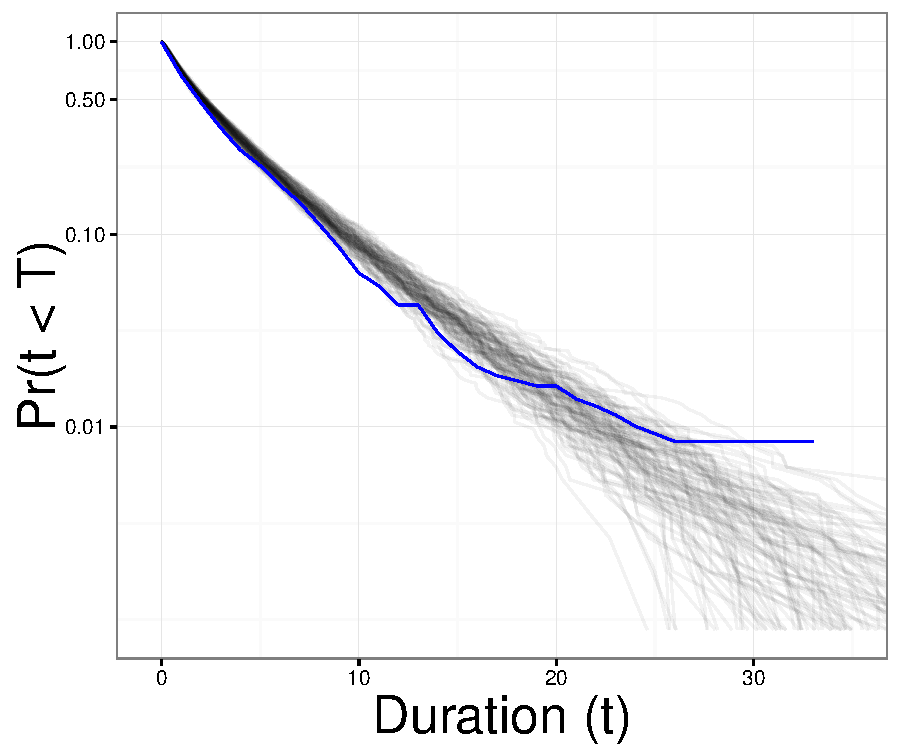
\includegraphics[height = 0.5\textheight,width=\textwidth,keepaspectratio=true]{figure/survival_curves}
  \caption{Comparison of the empirical estimate of \(S(t)\) (highlighted) versus estimates from 1000 posterior predictive data sets (black). \(S(t)\) corresponds to the probability that the age of a genus \(t\) is less than the genus' ultimate duration \(T\). The vertical axis is log10 transformed.}
  \label{fig:surv}
\end{figure}

\begin{figure}[ht]
  \centering
  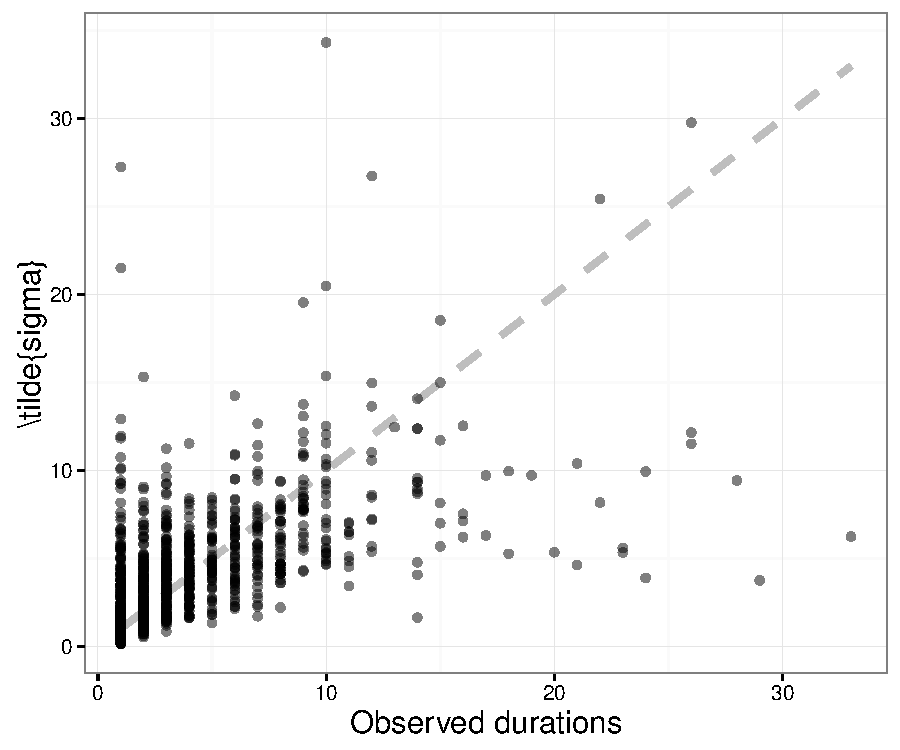
\includegraphics[height = 0.5\textheight,width=\textwidth,keepaspectratio=true]{figure/shotgun}
  \caption{Comparison of all observed genus durations in number of geological stages to the average posterior predictive estimates of \(\log(\sigma)\). The dashed, diagonal line correpsonds to \(x = y\).}
  \label{fig:shot}
\end{figure}


The cohort-level estimate of the effect of geographic range size indicates that as a taxon'sgeographic range increases, that taxon's duration is expected to increase (Table \ref{tab:param}). Given the estimates of \(\mu_{r}\) and \(\tau_{r}\), there is a less than 0.008\% (\(\pm 0.05\)) probability that this relationships would be reversed (\(\mathrm{Pr}\left(\mathcal{N}(\mu_{r}, \tau_{r}) > 0\right)\)). The between cohort variance in the cohort-specific estimates of the effect of geographic range \(\beta_{r}\) are the lowest of all the regression coefficients (Table \ref{tab:param}.

Body size is estimated to have no effect on taxon duration, with the estimate nearly centered at 0 (Table \ref{tab:param}). The variance between the cohort-specific estimates of the effect of body size \(\tau_{m}\) is found to be greater than the variance of between-cohort estimates of the effect of geographic range size \(\tau_{r}\). 

The group-level estimate of the effect of environmental preference is estimated from both \(\mu_{v}\) and \(\mu_{v^{2}}\). 

The estimate of \(\mu_{v}\) indicates that epicontinental favoring taxa are expected to have a greater duration than open-ocean favoring taxa. Additionally, given the estimate of between cohort variance \(\tau_{v}\), there is approximately 19\% (\(\pm 8 SD\)) probability that taxa favoring open-ocean environments would have a greater expected duration than taxa favoring epicontinental environments (\(\mathrm{Pr}\left(\mathcal{N}(\mu_{v}, \tau_{v}) > 0 \right)\)). Notice the direction of the inequality given the negative size in equation \ref{eq:sigma}. There is a high amount amount of between-cohort variation in estimates of \(\beta_{v}\) (Table \ref{tab:param}).

The estimate of \(\mu_{v^{2}}\) indicates that the overall relationship between environmental preference and \(\log(\sigma)\) is concave down (Fig. \ref{fig:env_mean}), with only a 1.9\% (\(\pm 2.4\)) probability that any given cohort is not concave down (\(\mathrm{Pr}\left(\mathcal{N}(\mu_{v^{2}}, \tau_{v^{2}})\right) < 0\)). As above, notice the direction of the inequality given the negative size in equation \ref{eq:sigma}. Given the estimate of \(\tau_{v^{2}}\), there is an expected high amount amount of between-cohort variation in estimates of \(\beta_{v^{2}}\) (Table \ref{tab:param}).

\begin{table}
  \centering
  \caption{Group-level estimates of the effects of biological traits on brachiopod generic survival. \(\mu\) values are the location parameters of the effects, while \(\tau\) values are the scale terms describing the variation between cohorts. The mean, standard deviation, 10th, 50th, and 90th quantiles of the posterior are presented.}
  \begin{tabular}{ l r r r r r }
    \hline
    parameter & mean & standard deviation & 10\% & 50\% & 90\% \\ 
    \hline
    \(\mu_{i}\) & -2.32 & 0.14 & -2.50 & -2.32 & -2.15 \\ 
    \(\mu_{r}\) & -0.76 & 0.11 & -0.91 & -0.76 & -0.62 \\ 
    \(\mu_{v}\) & -0.66 & 0.17 & -0.88 & -0.66 & -0.43 \\ 
    \(\mu_{v^{2}}\) & 2.88 & 0.31 & 2.48 & 2.88 & 3.27 \\ 
    \(\mu_{m}\) & 0.04 & 0.12 & -0.12 & 0.04 & 0.19 \\ 
    \(\tau_{i}\) & 0.50 & 0.10 & 0.37 & 0.49 & 0.63 \\ 
    \(\tau_{r}\) & 0.27 & 0.13 & 0.11 & 0.26 & 0.45 \\ 
    \(\tau_{v}\) & 0.76 & 0.16 & 0.56 & 0.74 & 0.97 \\ 
    \(\tau_{v^{2}}\) & 1.24 & 0.33 & 0.84 & 1.21 & 1.67 \\ 
    \(\tau_{m}\) & 0.47 & 0.12 & 0.33 & 0.47 & 0.63 \\ 
    \hline
  \end{tabular}
  \label{tab:param}
\end{table}


\begin{figure}[ht]
  \centering
  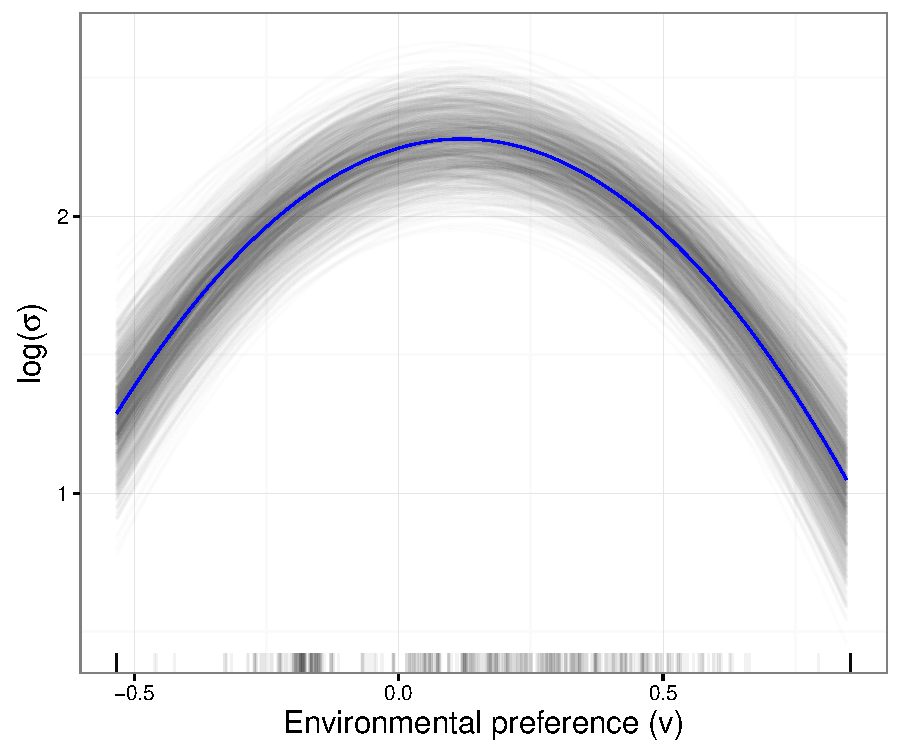
\includegraphics[height = 0.5\textheight,width=\textwidth,keepaspectratio=true]{figure/env_effect}
  \caption{The overall expected relationship between environmental affinity \(v_{i}\) and a \(\log(\sigma)\) when r = 0 and m = 0. Each grey line corresponds to a single draw from the posterior predictive distribution, while the highlighted line corresponds to the median of the posterior predictive distribution. The overall relationship is concave down with an optimum greater than 0, which means that taxa favoring epicontinental environments are expected to have longer durations than those favoring open-ocean environments.}
  \label{fig:env_mean}
\end{figure}



The cohort-specific estimates of all the regression coefficients demonstrate a lot of cohort to cohort variance, with no obvious trends. As indicated in Table \ref{tab:param} and detectable visually (Fig. \ref{fig:cohort_series}), the between-cohort estimates for \(\beta_{0}\), \(\beta_{r}\), and \(\beta_{m}\) all have much lower variance than the between-cohort estimates of both \(\beta_{v}\) and \(\beta_{v^{2}}\).

While most cohort-specific estimates are very similar to the overall cohort-level estimate there are a few notable excursions away from the overall mean (Fig. \ref{fig:cohort_series}). There are simultaneous excursions in both \(\beta_{0}\) and \(\beta_{v}\) for cohorts originating in the Giventian (387-382 My) and Frasnian (382-372 My) stages; both of which directly precede the end-Devonian mass extinction event at the Frasnian/Famennian boundary. These excusions indicate notably high extinction intensity faced by these cohorts along with an increase in expected duration for taxa favoring epicontinental environments over open-ocean ones.

Cohorts originating from the Silurian through the Early Devonian have a slightly lower extinction intensity than the overall mean; these are the from the Landovery (443-443 My) through the Emsian (407-393 My). This is also a time period where there is the lowest probability that epicontinental favoring taxa expected to have greater duration than open-ocean favoring taxa. Both the Silurian and Devonian periods are notable for having been periods with a mostly ``hothouse'' climate, with no polar icecaps and a high sea-level.
% Probability inflection point > 0 for cohorts 6 (Kantian) through 15 (Eifelian):
%   0.994, 0.988, 0.777, 0.262, 0.652, 0.648, 0.34, 0.848, 0.363, 0.996

\begin{figure}[ht]
  \centering
  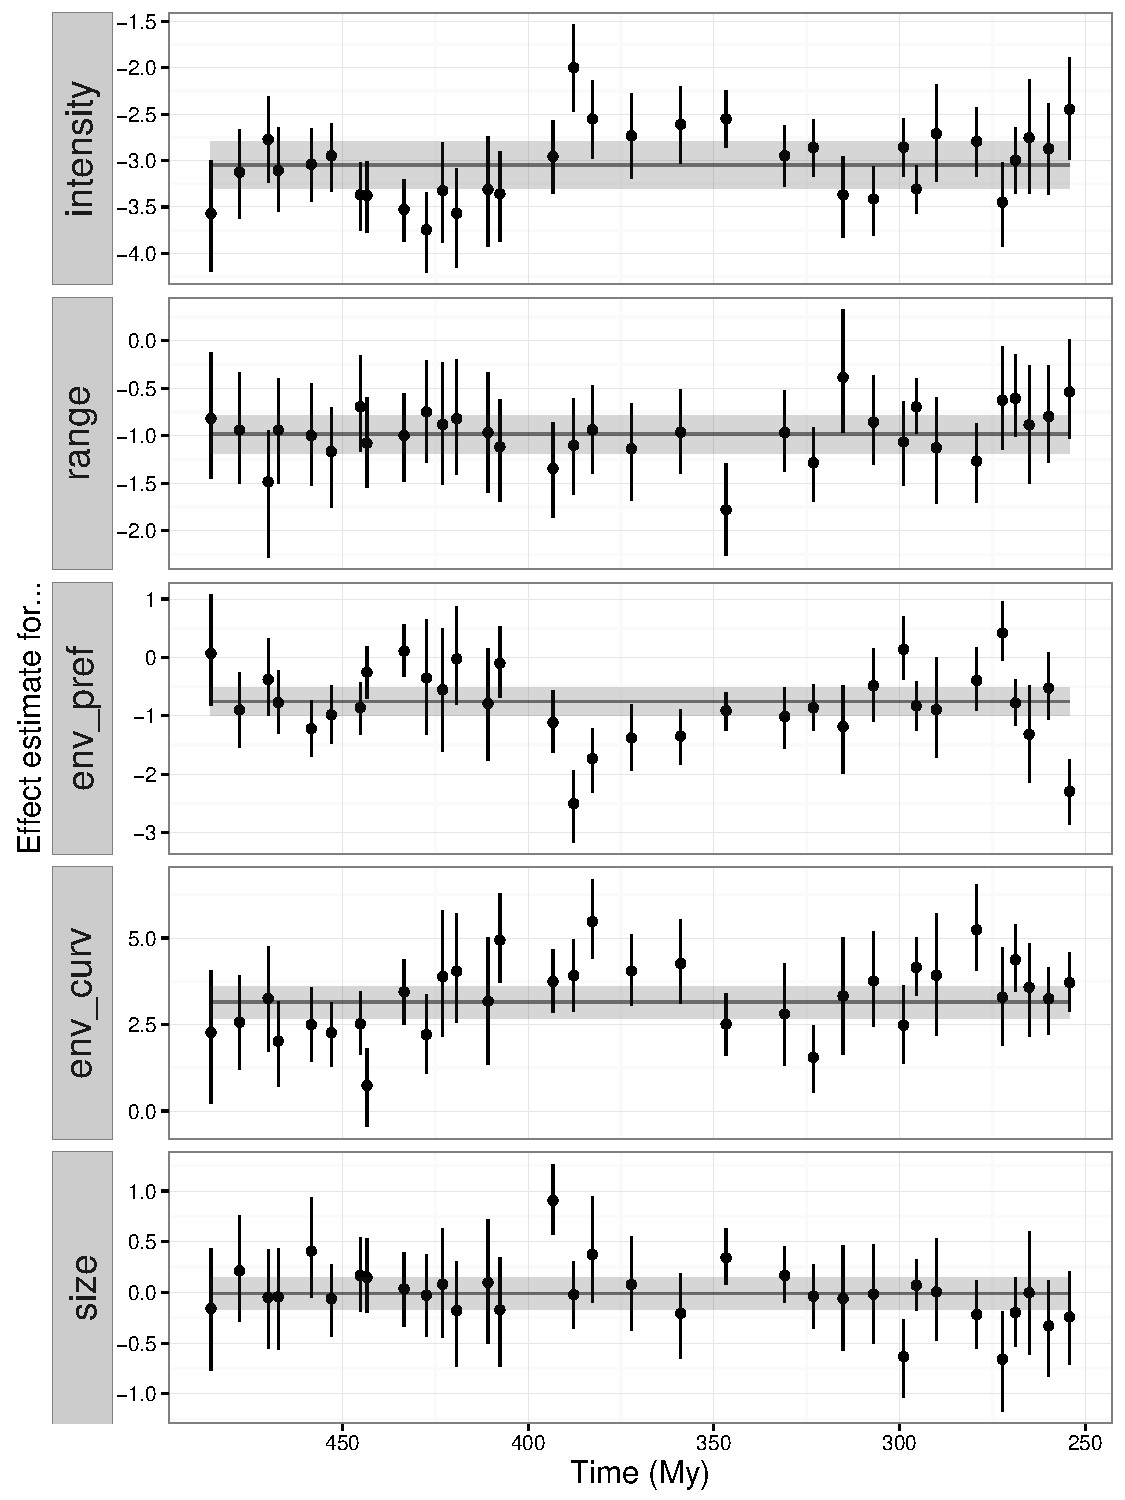
\includegraphics[width = \textwidth,height = \textheight,keepaspectratio=true]{figure/cohort_series}
  \caption{Comparison of cohort-specific estimates of \(\beta_{0}\), the effect of geographic range on extinction risk \(\beta_{r}\), the effect of environmental preference \(\beta_{v}\) and \(\beta_{v^{2}}\), and body size \(\beta_{m}\). Points correspond to the median of the cohort-specific estimate, along with 80\% credible intervals. Points are plotted at the midpoint of the cohorts stage of origination in millions of years before present (My). Black, horizontal lines are the overall estimates of covariate effects along with 80\% credible intervals (shaded).}
  \label{fig:cohort_series}
\end{figure}



% cohort-specific environmental effect
%   description of the variation in estimates
%   mass extinction boundaries
The cohort-specific relationships between environmental preference and \(\log(\sigma)\) were calculated from the estimates of \(\beta_{0}\), \(\beta_{v}\), and \(\beta_{v^{2}}\) (Fig. \ref{fig:env_cohort}) and reflect how these three parameters act in concert and not just individually (Fig. \ref{fig:cohort_series}). Beyond results already discussed above in the context of individual parameters, it is notable that the cohort originating in the Kungurian (279-272 My) has the most sharply curved appearance due to a high estimate \(\beta_{v^{2}}\) (Fig. \ref{fig:cohort_series}). This cohort expected to have the biggest different in extinction risk between environmtal generalists and specialists. The cohorts originating during the Emsian (407-393 My) and Frasnian (382 - 372 My) are tied for second for sharpness of curvature. The least sharply curved cohorts include those orignating during Tremadocian (484-477 My), Hirnantian (445-443 My), Llandovery (443-433 My), and Ludlow (427-423 My). Except for the Tremadocian cohort, all of these cohorts originate during the Silurian through the Early Devonian range identified earlier as having lower expected extinction intensity than what is expected from the group-level estimate.



\begin{figure}[ht]
  \centering
  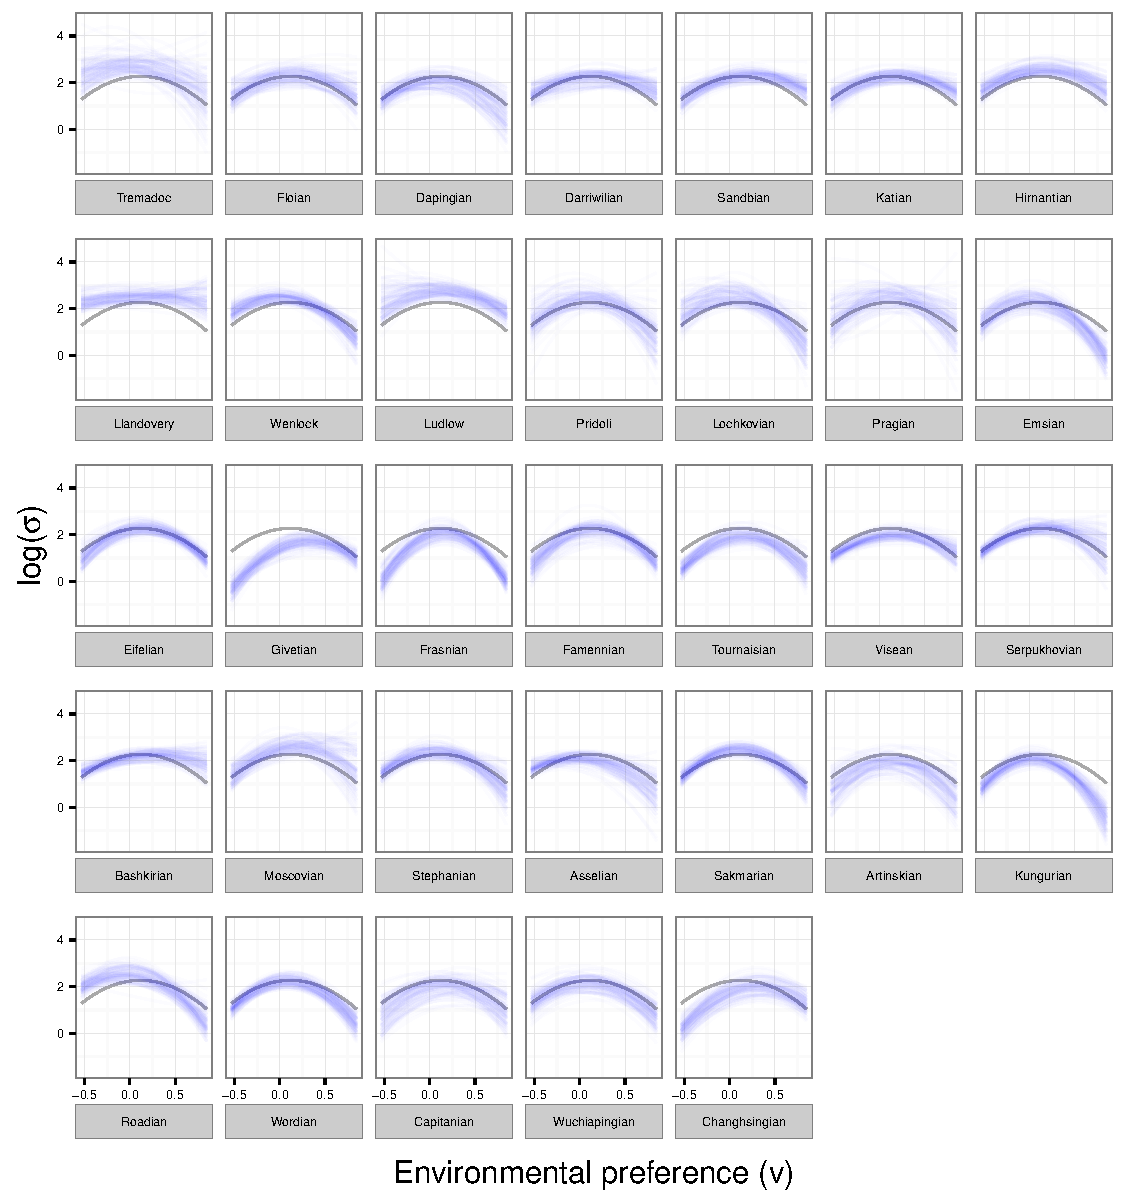
\includegraphics[width = \textwidth,height = \textheight,keepaspectratio=true]{figure/env_cohort}
  \caption{Comparison of origination cohort-specific (posterior predictive) estimates of the effect of environmental preference on \(\log(\sigma)\) to the mean overall estimate of the effect of environmental preference. Cohort-specific estimates are from 100 posterior predictive simulations across the range of (transformed and rescaled) observed values of enviromental preference. The oldest cohort is in the top-right and younger cohorts proceed left to right, with the youngest cohort being the right-most facet of the last row. Facet names correspond to the name of the stage in which that cohort originated.}
  \label{fig:env_cohort}
\end{figure}



The correlation in between cohort-specific estimates of the regression coefficients are estimated as the off-diagonal elements of the correlation matrix \(\Omega\). Only two of the elements of \(\Omega\) are distinguishable from 0: the correlation of \(\beta_{0}\) (extinction intensity) with both \(\beta_{r}\) and \(\beta_{v}\) (Fig. \ref{fig:cor_posterior}). 

There is an approximate 86\% probability that the cohort-specific estimates of baseline extinction intensity \(\beta_{0}\) and the effect of geographic range \(\beta_{r}\) are negatively correlated; this means that it is expected that for cohorts experiencing a lower extinction intensity the effect of geographic range inceases, and \textit{vice versa}. 

Similarly, there is an approximate 99.9\% probability that the cohort-specific estimates of \(\beta_{0}\) and \(\beta_{v}\) are negatively correlated; this means that as extinction intensity increases it is expected that epicontinental taxa become less favored over open-ocean environments. Again, note that there is a 19\% (\(\pm 8.1 SD\) probability that, for any given cohort, open-ocean environments will be favored.

Estimates of \(\beta_{r}\) and \(\beta_{v}\) are themselves not correlated, as there is only an approximate 68\% probability of a positive correlation. The lack of cross-correlation may be caused by the much higher between-cohort variance of the effect of environmental preference \(\tau_{v}\) than the very small between-cohort variance in the effect of geographic range \(\tau_{r}\) (Table \ref{tab:param}). The effect of geographic range might simply not vary enough relative to each other to detect a correlation with the much noiser effect of environmental preference.

\begin{figure}[ht]
  \centering
  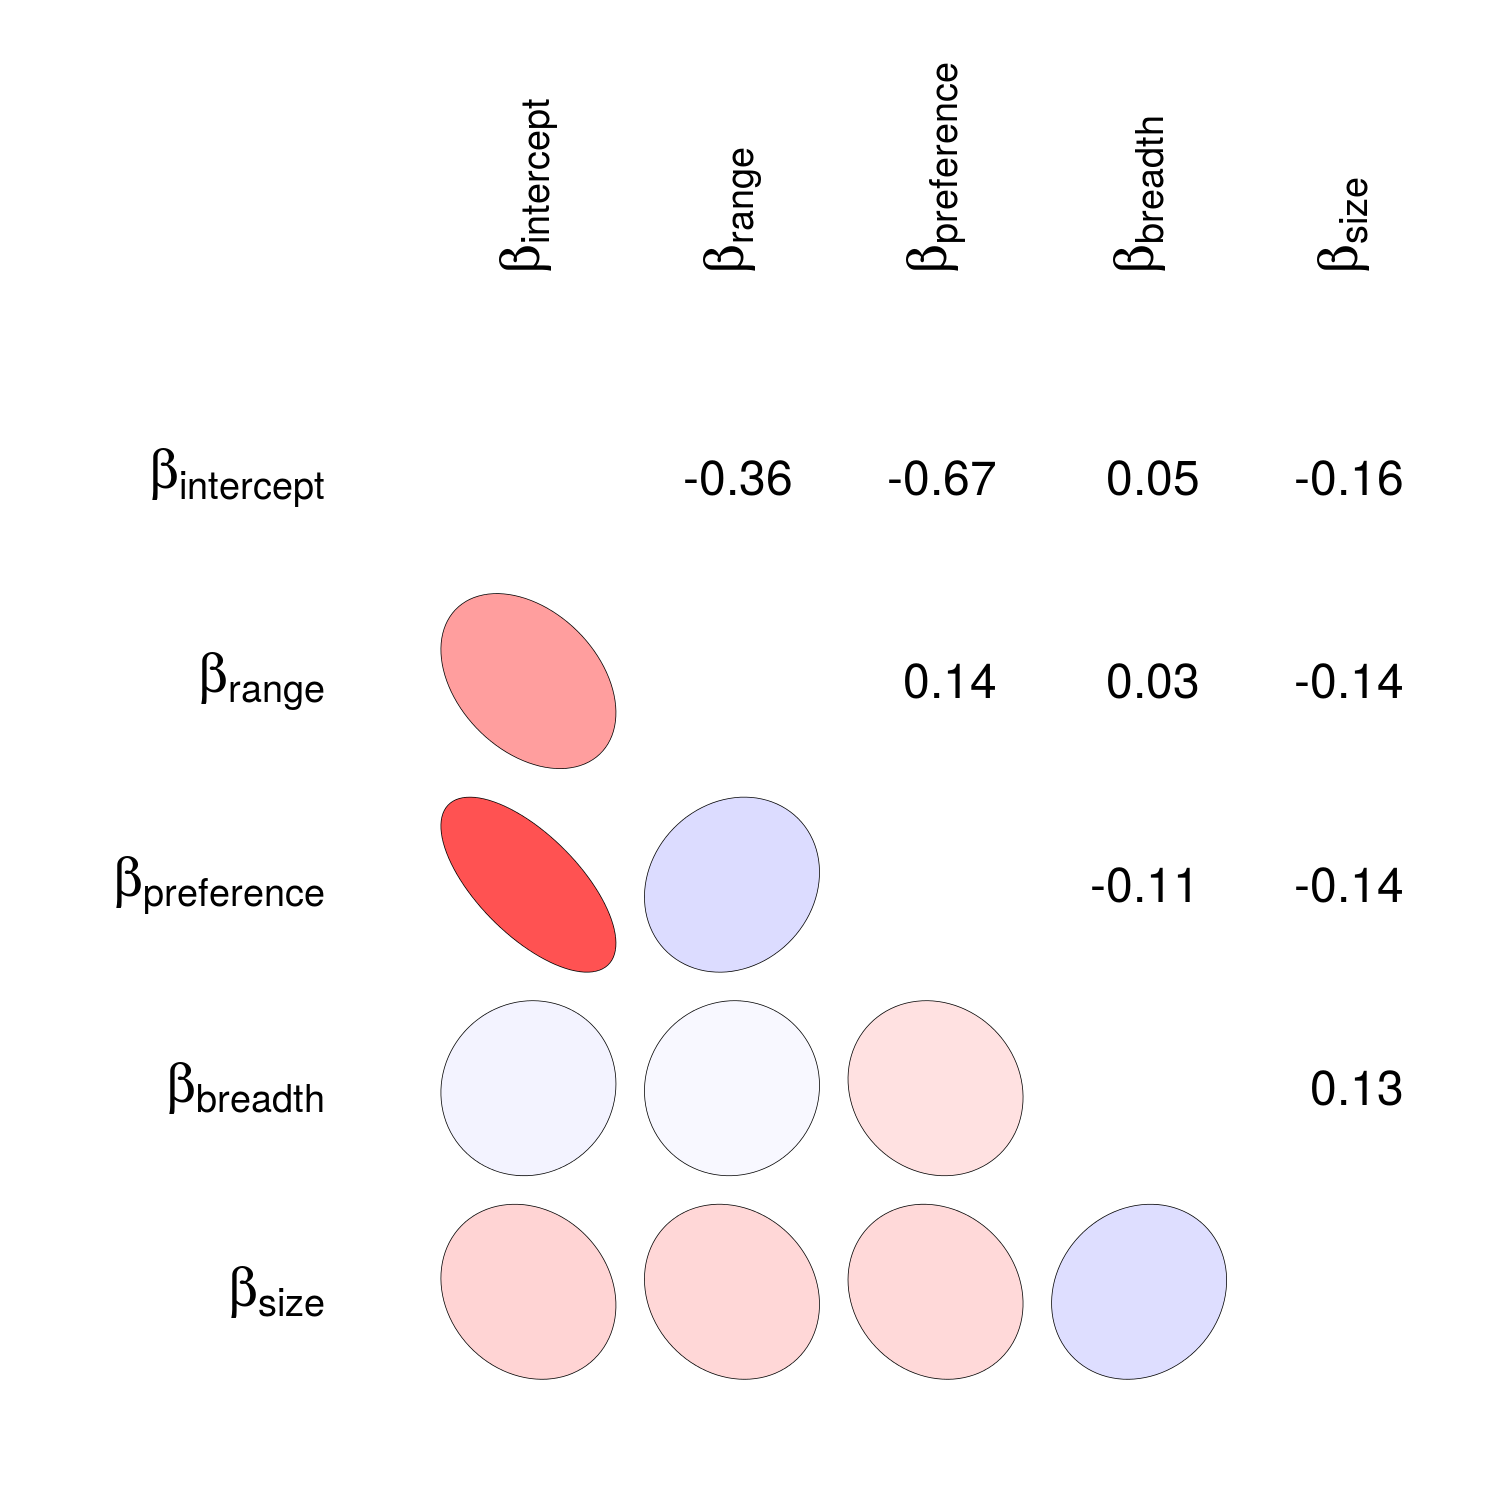
\includegraphics[height = 0.8\textheight,width=\textwidth,keepaspectratio=true]{figure/wei_cor_heatmap}
  \caption{Mixed graphical and numerical representation of the correlation matrix \(\Omega\) of variation in cohort-specific covariate estimates. These correlations are between the estimates of the cohort-level effects of covariates, along with intercept/baseline extinction risk. The median estimates of the correlations are presented numerically (upper-triangle) and as idealized ellipses representing that much correlation (lower-triangle).}
  \label{fig:cor_posterior}
\end{figure}





\section{Discussion}

% discussion of results and their interpretation

% sampling and duration
%   y = y^{*} - 2(average gap duration)
%   difficulty including 1, 2, or even 3 duration taxa
%     no gaps
%   removing would remove so much valuable information
%     law of constant extinction/surival analysis : young observations are really important
%       truncation by still tremendous loss of data
%   simplify by making all taxa have sample average gap -- makes sampling have no effect
%     equal for all
%   Solow and Smith and Tanja's BDSS use duration / number occurrences
%     MLE
%     how much would this actually affect duration when resolution is stage

% environmental preference
%   are generalists older because they are generalists or because of adaptation facilitating persistence?
%     Harnik + Simpson + Hopkins
%   do things ``start'' specialist then ``become'' generalists over time/their duration
%     (macro)evolution and adaptation
%     persistance

% intensity and selectivity
%   negative cor beta_0 and beta_r
%   negative cor beta_0 and beta_v


% discussion of context of study
%   defense
%     species:genus?
%     difficulty towards tails, but that's to be expected
%       this model is about expectations, not tails/extreme events
%       this model is ok for the main part of the data
%       though, of course, this model has a long way to go (all models are false)
The use of genera as the unit of the study and how to exactly interpret the effects of the biological traits is a remaining concern. For example, if any of the traits analyzed here are associated with increases in speciation rates, this might increase the duration of genera through self-renewal \citep{Raup1991b,Raup1994}, which would be an example of the difference in biological pattern between species and genera \citep{Jablonski1987,Jablonski2007,Jablonski2008a}. This could lead to a trait appearing to decrease generic level extinction risk by increasing species level origination rate instead of decreasing species level extinction risk. However, given the nature of the fossil record and maintaining a minimum level of data consistency/quality, there is no simple solution to decreasing this uncertainty in the interpretations of how the biological traits studied at the genus-level may translate to the species-level.

% future direction
The model used here could be improved through either increasing the number of analyzed taxon traits, expanding the hierarchical structure of the model to include other major taxonomic groups of interest, and the inclusion of explicit phylogenetic relationships between the taxa in the model as an additional hierarchical effect. An example taxon trait that may be of particular interest is the affixing strategy or method of interaction with the substrate of the taxon, which has been found to be related to brachiopod survival where, for cosmopolitan taxa, taxa that are attached to the substrate are expected to have a greater duration than those that are not \citep{Alexander1977}.

%   comparison with other major groups in hierarchical model
It is theoretically possible to expand this model to allow for comparisons within and between major taxonomic groups. This approach would better constrain the brachiopod estimates while also allowing for estimation of similarities and differences in cross-taxonomic patterns. The major issue surrounding this particular expansion involves finding an similarly well sampled taxonomic group that is present during the Paleozoic. Example groups include Crinoidea, Ostracoda, and other members of the ``Paleozoic fauna'' \citep{SepkoskiJr.1981a}.

Taxon traits like environmental preference or geographic range \citep{Jablonski1987,Hunt2005b} are most likely heritable, at least phylogenetically \citep{Lynch1991,Housworth2004}. Without phylogenetic context, this analysis assumes that differences in extinction risk between taxa are independent of the shared evolutionary history of those  taxa \citep{Felsenstein1985b}. In contrast, the origination cohorts only capture shared temporal context. For example, if taxon duration is phylogenetically heritable, then closely related taxa may have more similar durations as well as more similar biological traits. Without taking into account phylogenetic similarity the effects of these biological traits would be inflated solely due to inheritance. The inclusion of phylogenetic context as an additional individual-level hierarchical effect independent of origination cohort would allow for determining how much of the observed variability is due to shared evolutionary history versus shared temporal context versus actual differences associated with biological traits \citep{Smits2015}. 

% concluding statements
% TODO
%In summary, patterns of Paleozoic brachiopod survival were analyzed using a fully Bayesian hierarchical survival modelling approach while also eschewing the traditional separation between background and mass extinction. I find that as baseline extinction risk increases, the form of the selectivity of extinction changes such that during periods of low extinction risk the effect environmental preference is expected to change from nonlinear to potentially linear or even absent while the effect of geographic range increases. In particular, the correlation between the effect of geographic range and the curvature of the effect of environmental preference on taxon survival supports the hypothesis that during periods of high extinction intensity of the effect of geographic range effectively washes out the effects of other biological traits \citep{Jablonski1987,Raup1991b}. Finally, I find weak support for ``survival of the unspecialized'' \citep{Simpson1944,Liow2004a,Liow2007b,Nurnberg2013a,Nurnberg2015} as a general characterization of the effect of environmental preference on extinction risk (Fig. \ref{fig:env_mean}), most origination cohorts conforming to this hypothesis (Fig. \ref{fig:env_cohort}). 


\section*{Acknowledgements}
I would like to thank K. Angielzcyk, M. Foote, P. D. Polly, R. Ree, and G. Slater for helpful discussion during the conception of this study. I'd also like to thank D. Bapst, N. Pierrehumbert and M. Villarosa Garcia for additional comments. Additionally, thank you A. Miller for the epicontinental versus open-ocean assignments. This entire study would would not have been possible without the Herculean effort of the many contributors to the Paleobiology Database. In particular, I would like to thank J. Alroy, M. Aberhan, D. Bottjer, M. Clapham, F. F\"{u}rsich, N. Heim, A. Hendy, S. Holland, L. Ivany, W. Kiessling, B. Kr\"{o}ger, A. McGowan, T. Olszewski, P. Novack-Gottshall, M. Patzkowsky, M. Uhen, L. Villier, and P. Wager. This work was supported by a NASA Exobiology grant (NNX10AQ446) to A. Miller and M. Foote. I declare no conflicts of interest. This is Paleobiology Database publication XXX.

\clearpage

\bibliographystyle{evolution}
\bibliography{newbib,packages}

\clearpage



\end{document}

